% !TEX root = paper.tex

\section {Results}
\label{sec:results}

\begin{figure}[!hbt]
	\centering
	\subfigure{ 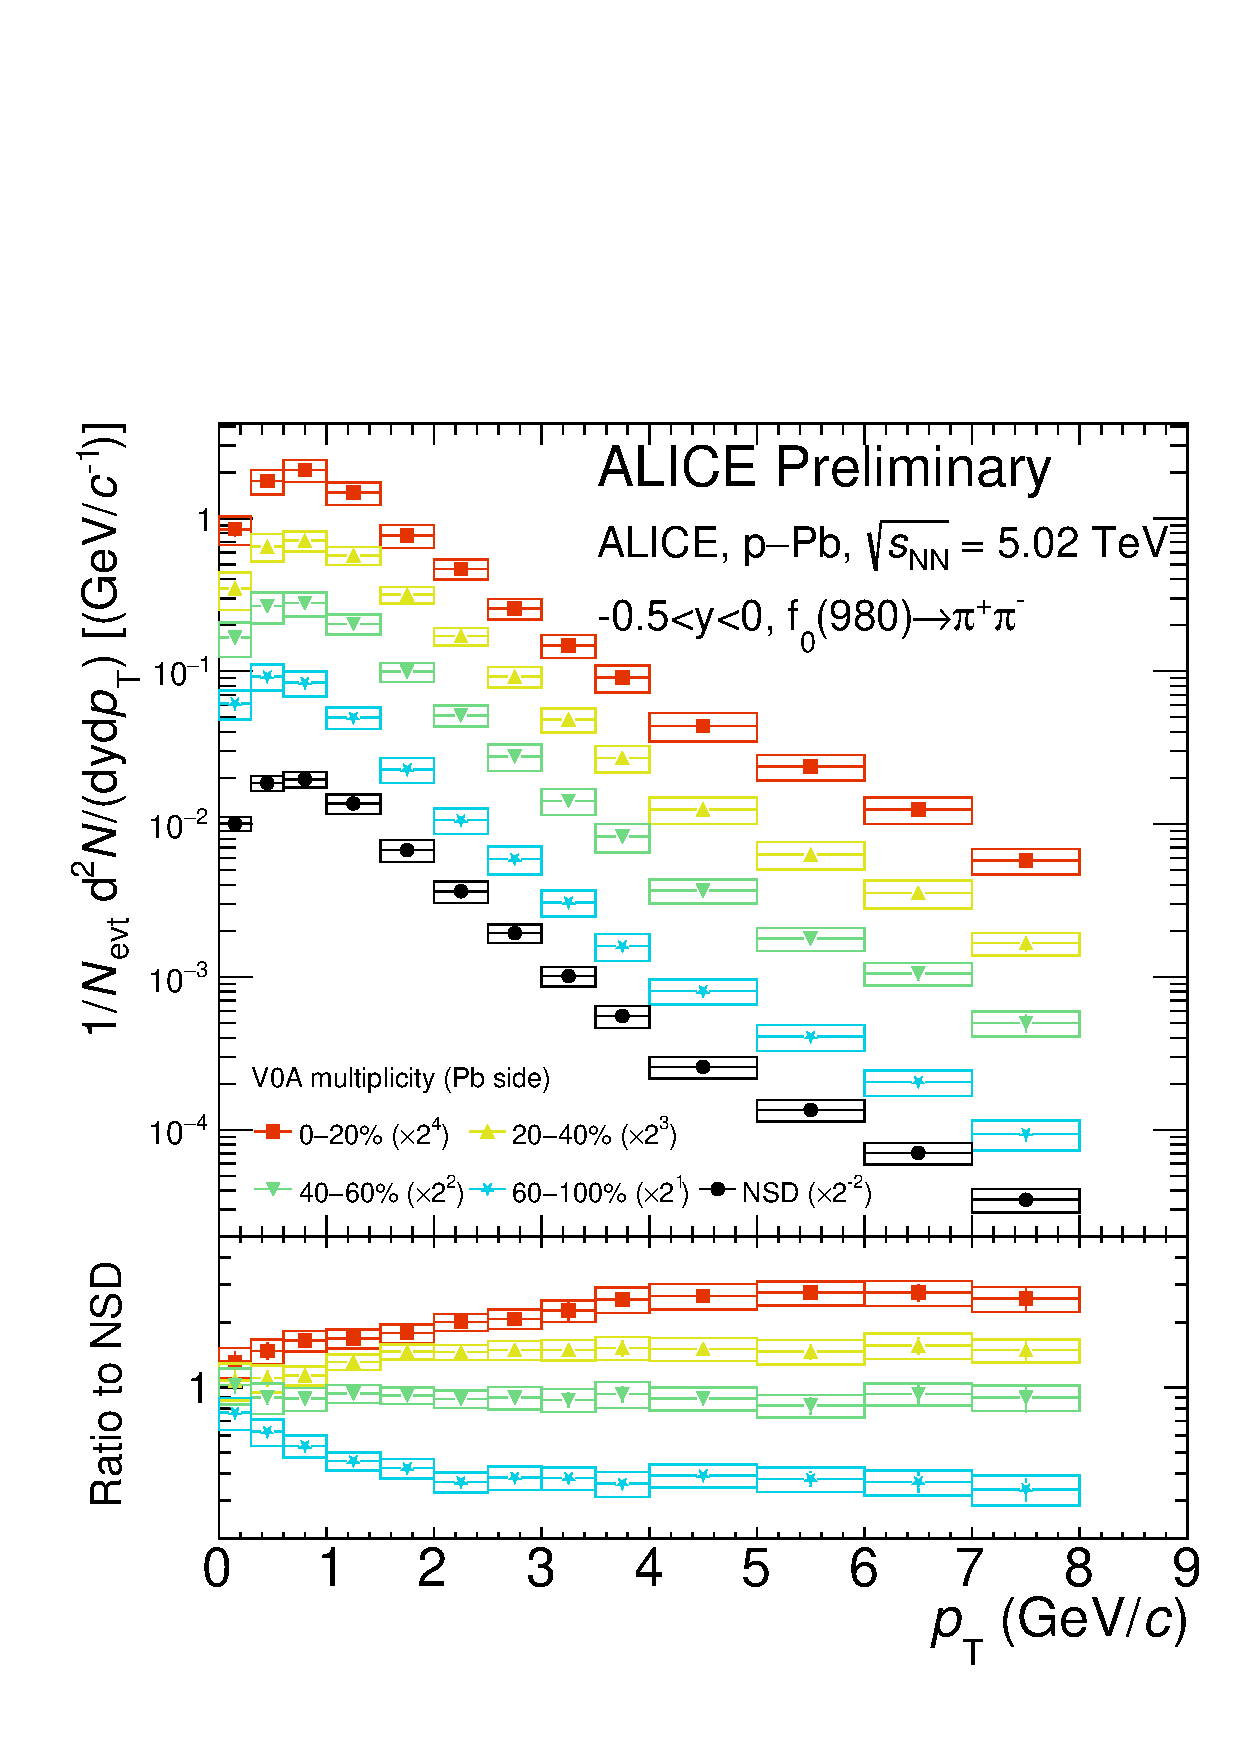
\includegraphics[width=0.6 \textwidth]{figures/Fig2_pt_all.pdf} }
	\caption{ Transverse momentum spectra of \fzero~in p--Pb collisions at \snn~=~5.02~TeV for different multiplicity classes, which are scaled for visibility. Statistical and systematic uncertainties are shown as error bars and boxes, respectively. The lower panel shows the ratios of the specific spectra to the NSD spectrum. }
	\label{fig:pt}
\end{figure}

Figure~\ref{fig:pt} shows the $p_{\mathrm{T}}$ spectra of \fzero~in p--Pb collisions at \snn~=~5.02~TeV measured in the range of 0~$<p_{\mathrm{T}}<$~8~GeV/$c$ for different multiplicity classes and non-single diffractive (NSD) events. Each spectrum is scaled with the number denoted in the figure for visibility. The lower panel of Fig.~\ref{fig:pt} shows the ratios of each $p_{\mathrm{T}}$ spectrum to the NSD spectrum. The systematic uncertainties of the ratios are estimated by propagating the multiplicity-uncorrelated uncertainties on the single spectrum. For $p_{\mathrm{T}}<$~4~GeV/$c$, the hardening of the $p_{\mathrm{T}}$ spectrum from low- to high-multiplicity events is clearly seen, while the same shape is visible at high $p_{\mathrm{T}}>$~4~GeV/$c$. Such trends can be also observed in other hadrons~\cite{Tsallis:1987eu}.

\begin{table}[h!]
\caption{The values of d$N$/d$y$ and mean $p_{\mathrm{T}}$ $\left( \left\langle p_{\mathrm{T}} \right\rangle \right)$ measured in p--Pb collisions at \snn~=~5.02~TeV for different multiplicity classes. The first and second uncertainties represent the statistical and systematic uncertainties, respectively. In each entry the first uncertainty is statistical and the second one is systematic. }
\centering
\begin{tabular}{ccc}
\hline 
Multiplicity class (V0A) & d$N$/dy & $\left\langle p_{\mathrm{T}} \right\rangle$ (GeV/$c$) \\ \hline
0--20\% & 0.206$\pm$0.005$\pm$0.014 & 1.287$\pm$0.034$\pm$0.010 \\
20--40\% & 0.153$\pm$0.004$\pm$0.010 & 1.250$\pm$0.029$\pm$0.082 \\
40--60\% & 0.113$\pm$0.002$\pm$0.008 & 1.142$\pm$0.025$\pm$0.088 \\
60--100\% & 0.064$\pm$0.001$\pm$0.005 & 0.999$\pm$0.014$\pm$0.080 \\
\hline
\end{tabular}
\label{tab:ymp}
\end{table}

Table~\ref{tab:ymp} shows the integrated yield (d$N$/d$y$) and mean $p_{\mathrm{T}}$ $\left( \left\langle p_{\mathrm{T}} \right\rangle \right)$ of \fzero~for different multiplicity classes in p--Pb collisions at \snn~=~5.02~TeV. The d$N$/d$y$ linearly increases with the multiplicity, while the $\left\langle p_{\mathrm{T}} \right\rangle$ concavely increases with the multiplicity. 

\begin{figure}[!hbt]
	\centering
	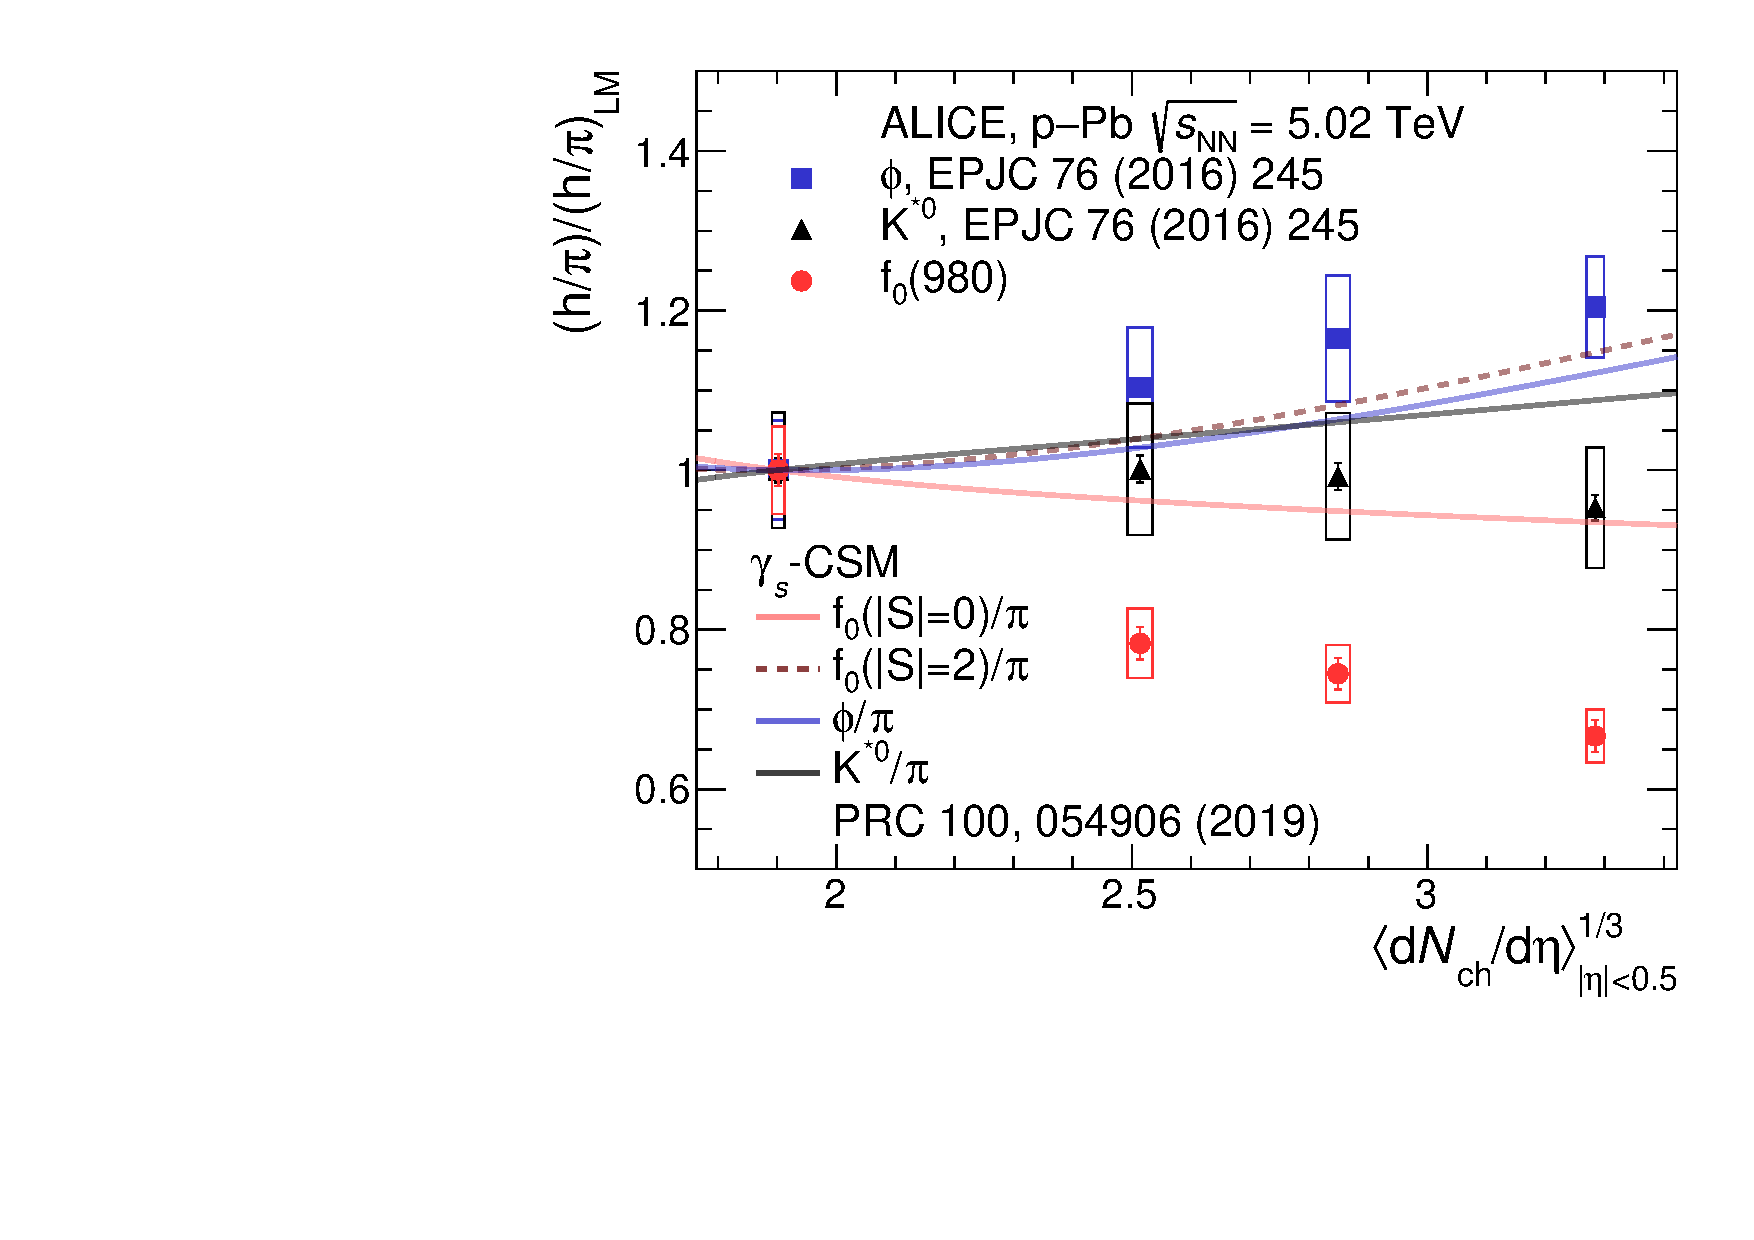
\includegraphics[width=0.49 \textwidth]{figures/Fig4_dr_pion_addCSM_addpar.pdf} 
        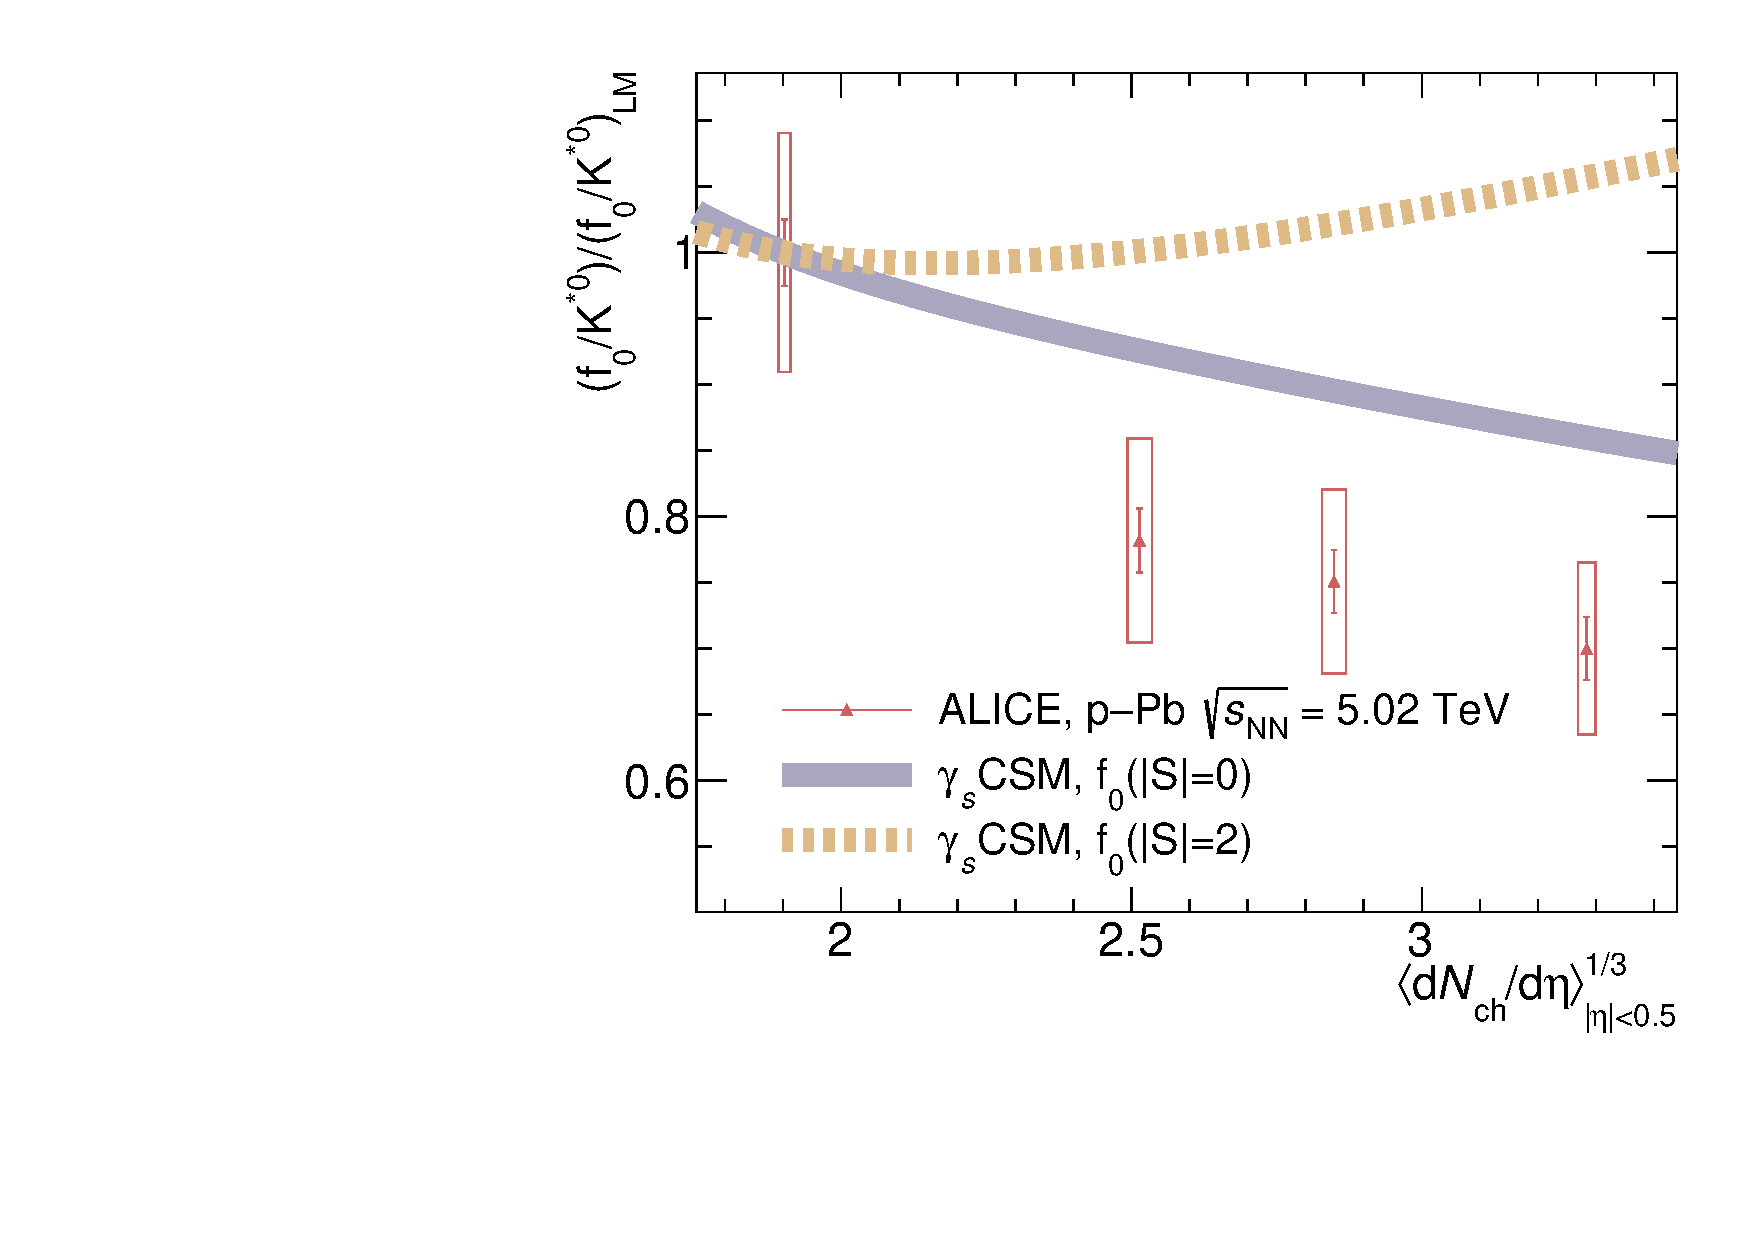
\includegraphics[width=0.49 \textwidth]{figures/Fig4_dr_kstar_addCSM.pdf} 
	\caption{ Double ratios of $\phi$, $\rm{}K^{*0}$(892), and \fzero~to $\pi$ (left) and \fzero~to $\rm{}K^{*0}$(892) (right) as a function of charged-particle multiplicity elevated to 1/3. The ratios are divided by the ratio in low-multiplicity (LM) events to make the first point unity and reduce systematic uncertainties. Predictions from the Canonical statistical model are represented with lines. }
	\label{fig:f0piAddCSM}
\end{figure}

The left panel of figure~\ref{fig:f0piAddCSM} shows the double ratios of different particles to charged pion yields as a function of charged-particle multiplicity elevated to 1/3 in p--Pb collisions at \snn~=~5.02~TeV. The charged-particle multiplicity is measured using the V0A detector. The systematic uncertainty of the double ratio is calculated with uncorrelated uncertainties only. The pion, $\rm{}K^{*0}$, and $\phi$ mesons can be classified according to their lifetimes and whether they contain (anti-) strange quarks. The strangeness enhancement and rescattering effects can be studied by comparing the yield of particles with different characteristics. The ratio of $\phi$ to $\pi$ increases with the multiplicity, which is consistent with the observation of the strangeness enhancement~\cite{ALICE:2016fzo}. On the other hand, the ratio of $\rm{}K^{*0}$ to $\pi$ is flat with the increasing multiplicity even if $\rm{}K^{*0}$ includes one strange quark. The flat trend could be explained by two competing effects, the strangeness enhancement and rescattering effects, as the lifetime of $\rm{}K^{*0}$ is 4.2~fm/$c$~\cite{ParticleDataGroup:2020ssz}. The ratio of \fzero~to $\pi$ decreases as the multiplicity increases because of the shorter lifetime of \fzero, suggesting rescattering effects for \fzero. Predictions of the ratio of \fzero~to $\pi$ are shown in lines for different hidden strangeness assumptions for \fzero~by $\gamma_{s}$-Canonical Statistical Model (CSM)~\cite{Vovchenko:2019kes}, which considers system-size-dependent hadrochemistry at vanishing baryon density with local conservation of electric charge, baryon density, and strangeness, while allowing for undersaturation of strangeness. Note that $\gamma_{s}$ is the parameter for the undersaturation of strangeness derived from measured particle yields. The CSM hypothesis with 2 hidden strange quarks predicts an increase of the ratio, contrarily to what observed experimentally. Moreover, the CSM with zero hidden strangeness estimates the ratio to be flat, which overestimates the data. Such a difference is attributed to no rescattering effects in the CSM. The prediction of the CSM for the ratio of $\phi$ to $\pi$ nicely reproduces the increasing trend of measured data with the increasing multiplicity. However, the CSM overestimates the ratio of $\rm{}K^{*0}$ to $\pi$ because the modification of $\rm{}K^{*0}$ yields due to rescattering effects is not implemented in the CSM.

The right panel of figure~\ref{fig:f0piAddCSM} shows the double ratio of \fzero~to $\rm{}K^{*0}$ yields as a function of charged-particle multiplicity elevated to 1/3 in p--Pb collisions at \snn~=~5.02~TeV and predictions from the CSM with different hidden strangeness assumptions. The lifetimes of \fzero~and $\rm{}K^{*0}$ are estimated to be comparable, indicating that rescattering effects would not be much different. Hence, the ratio is expected to be weakly affected by rescattering effects. The ratio decreases with increasing multiplicity that is qualitatively described with the zero-hidden-strangeness assumption and can be explained by the strangeness enhancement of the $\rm{}K^{*0}$ yield. The CSM prediction with the two-hidden-strangeness assumptions is mildly increasing as the multiplicity increases, a trend that is opposite to the experimental result as shown in Fig.~\ref{fig:f0piAddCSM}. Therefore, the decreasing trend of the ratio of \fzero~to $\rm{}K^{*0}$ can suggest no effective strangeness enhancement for the \fzero.

\begin{figure}[!hbt]
	\centering
	\subfigure{ 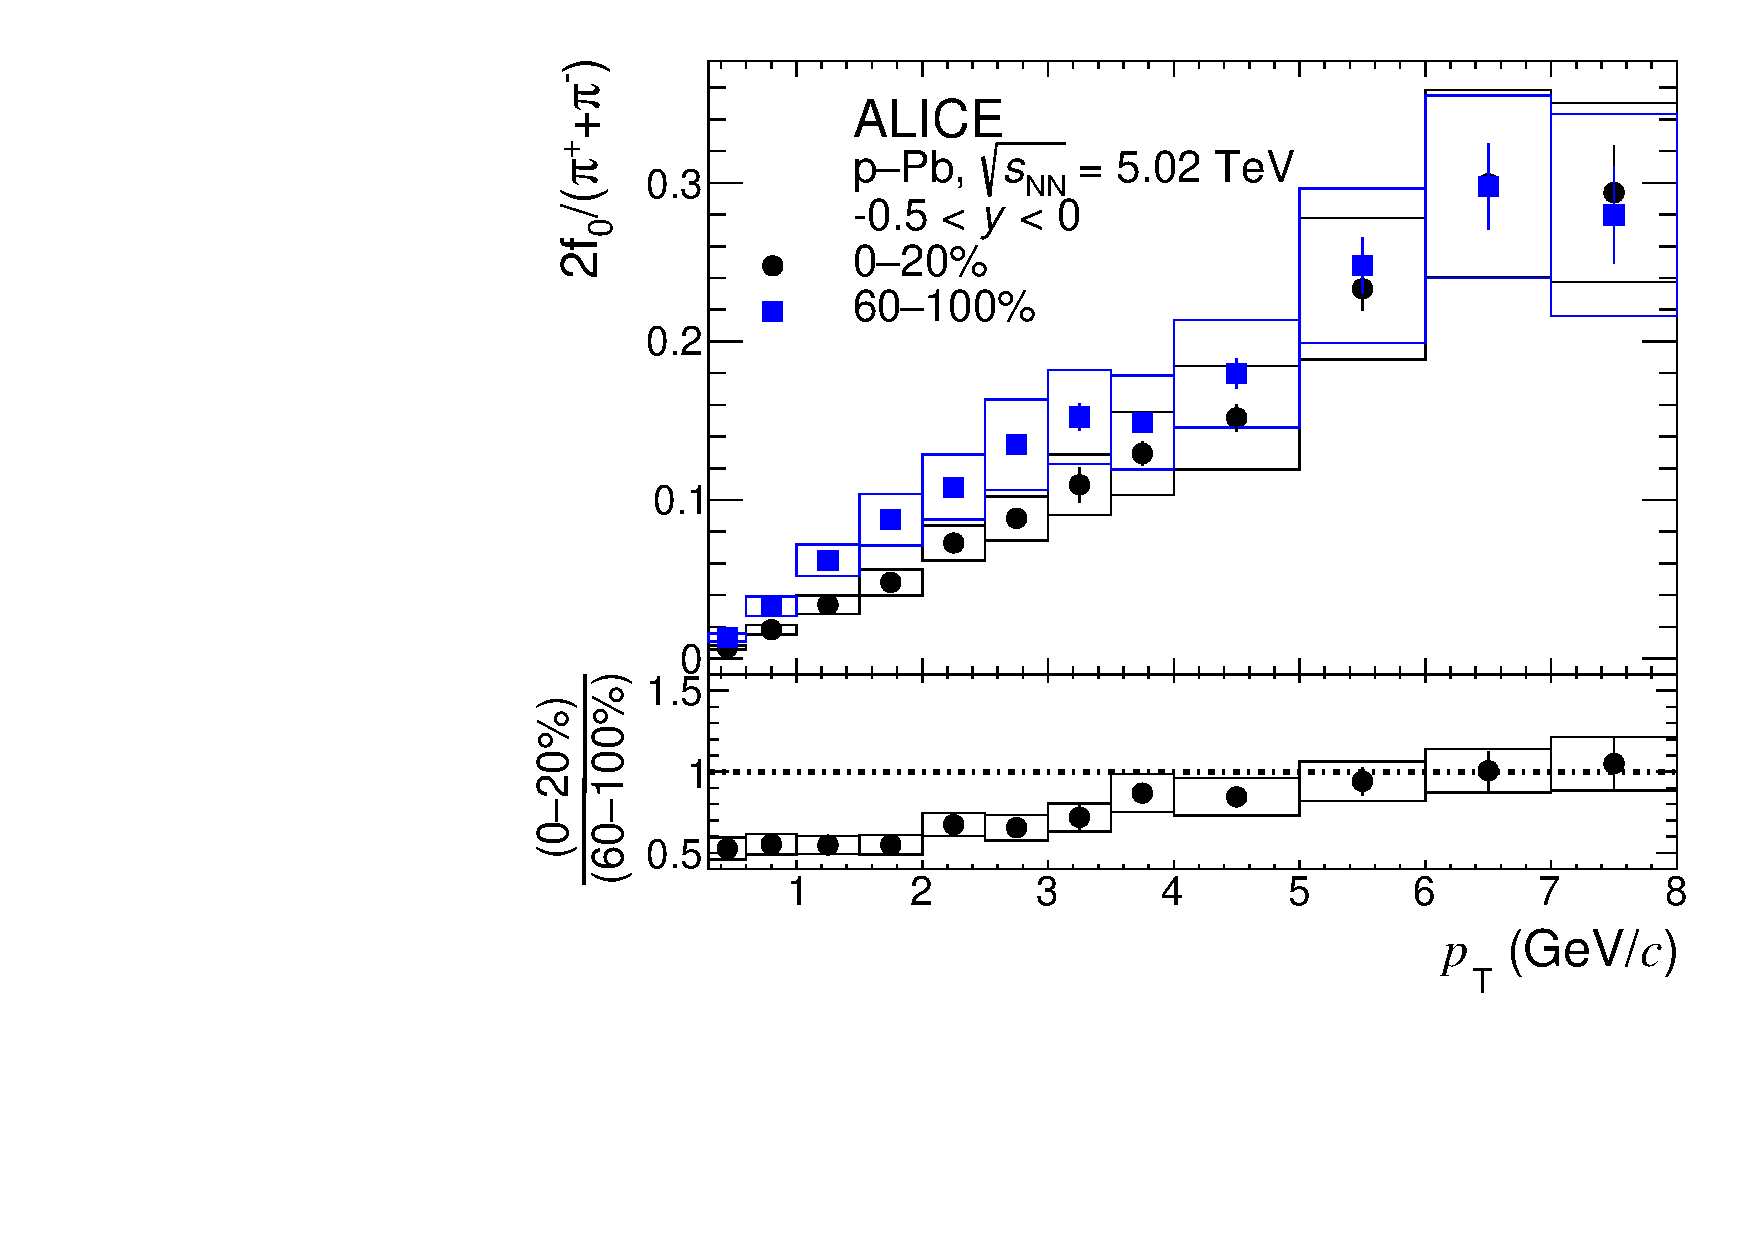
\includegraphics[width=0.6 \textwidth]{figures/Fig5_DR_pt_pion.pdf} }
	\caption{ The particle yield ratios of \fzero~to $\pi$ as a function of $p_{\rm{T}}$ in high-multiplicity (circles) and low-multiplicity (triangles) p--Pb collisions at \snn~=~5.02~TeV. The lower panel shows the double ratio of \fzero/$\pi$ between the high-multiplicity and low-multiplicity events. }
	\label{fig:f0piPt}
\end{figure}

Figure~\ref{fig:f0piPt} shows the $p_{\mathrm{T}}$-differential particle yield ratio of \fzero~to $\pi$ in high-multiplicity (HM) and low-multiplicity (LM) p--Pb collisions at \snn~=~5.02~TeV. The ratios are consistent within one sigma in $p_{\mathrm{T}}>$~4~GeV/$c$, while the double ratio of HM to LM is suppressed at a lower $p_{\mathrm{T}}$ as shown in the lower panel of Fig.~\ref{fig:f0piPt}. In the double ratio, the correlated uncertainties across multiplicity classes cancel. The $p_{\mathrm{T}}$ dependence of the double ratio indicates that the suppression of the integrated yield is an effect of the low $p_{\mathrm{T}}$ ($p_{\mathrm{T}}<$~4~GeV/$c$), which shows the same $p_{\mathrm{T}}$ dependence like the suppression of the $\rm{}K^{*0}/K$~\cite{ALICE:2019etb}.

\begin{figure}[!hbt]
	\centering
	\subfigure{ 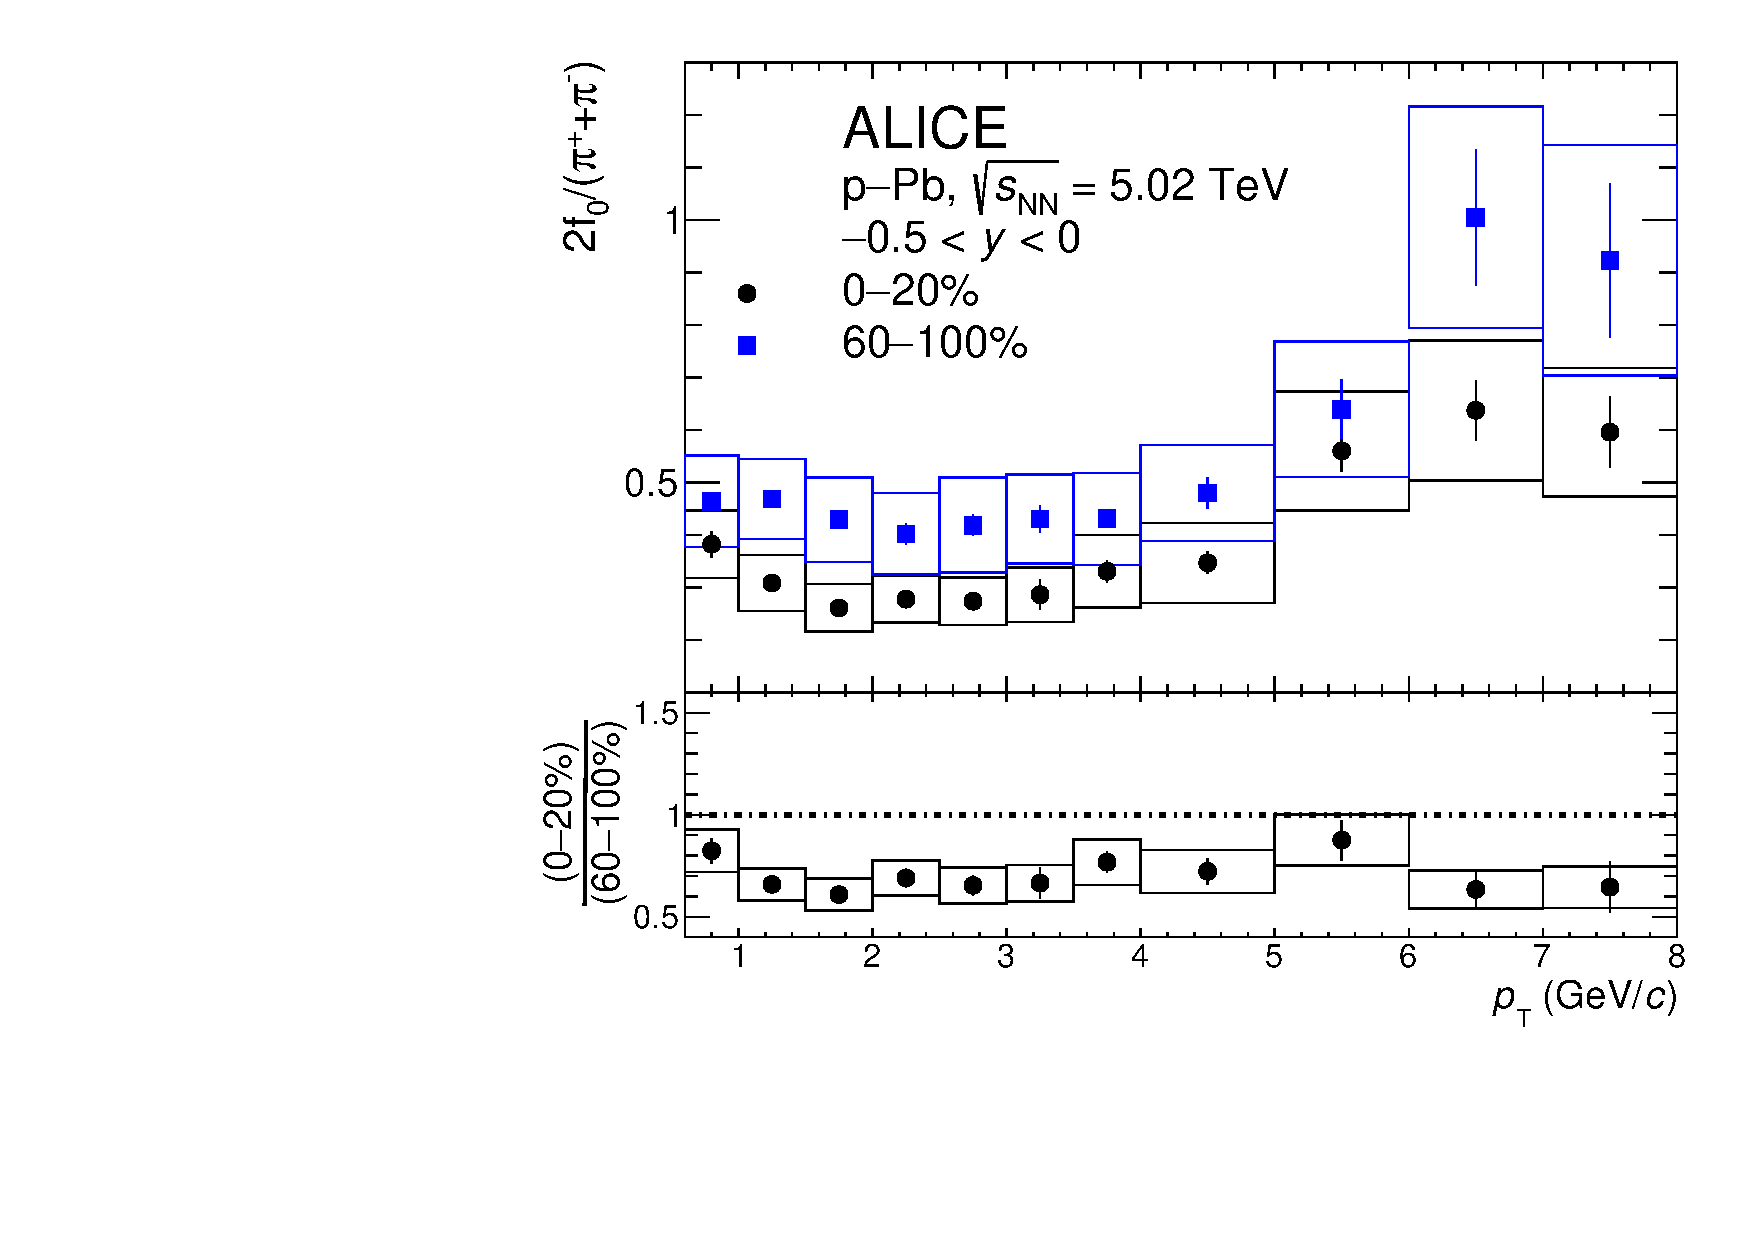
\includegraphics[width=0.6 \textwidth]{figures/Fig6_DR_pt_kstar.pdf} }
	\caption{The particle yield ratio of \fzero~to $\rm{}K^{*0}$(892) as a function of $p_{\rm{T}}$ in high-multiplicity (circles) and low-multiplicity (triangles) p--Pb collisions at \snn~=~5.02~TeV. The lower panel shows the double ratio of high-multiplicity to low-multiplicity \fzero/$\rm{}K^{*0}$(892).  }
	\label{fig:f0KsPt}
\end{figure}

Figure~\ref{fig:f0KsPt} shows $p_{\mathrm{T}}$-differential particle yield ratio of \fzero~to $\rm{}K^{*0}$ in HM and LM p--Pb collisions at \snn~=~5.02~TeV. The ratio from HM events is lower than that of LM events in the entire $p_{\mathrm{T}}$ range, which is different from $\rm{}K^{*0}/K$ or \fzero/$\pi$. The different $p_{\mathrm{T}}$ dependence of the double ratio indicates that other effects, rather than rescattering effects, are present. For instance, the enhancement of $\rm{}K^{*0}$ yield due to the strangeness enhancement can explain the suppression in the entire $p_{\mathrm{T}}$ range, while no strangeness enhancement for \fzero~yield. As a result, the decreasing trend of the ratio in higher multiplicity events suggests no strange quark in \fzero.

\begin{figure}[!hbt]
	\centering
	\subfigure{ 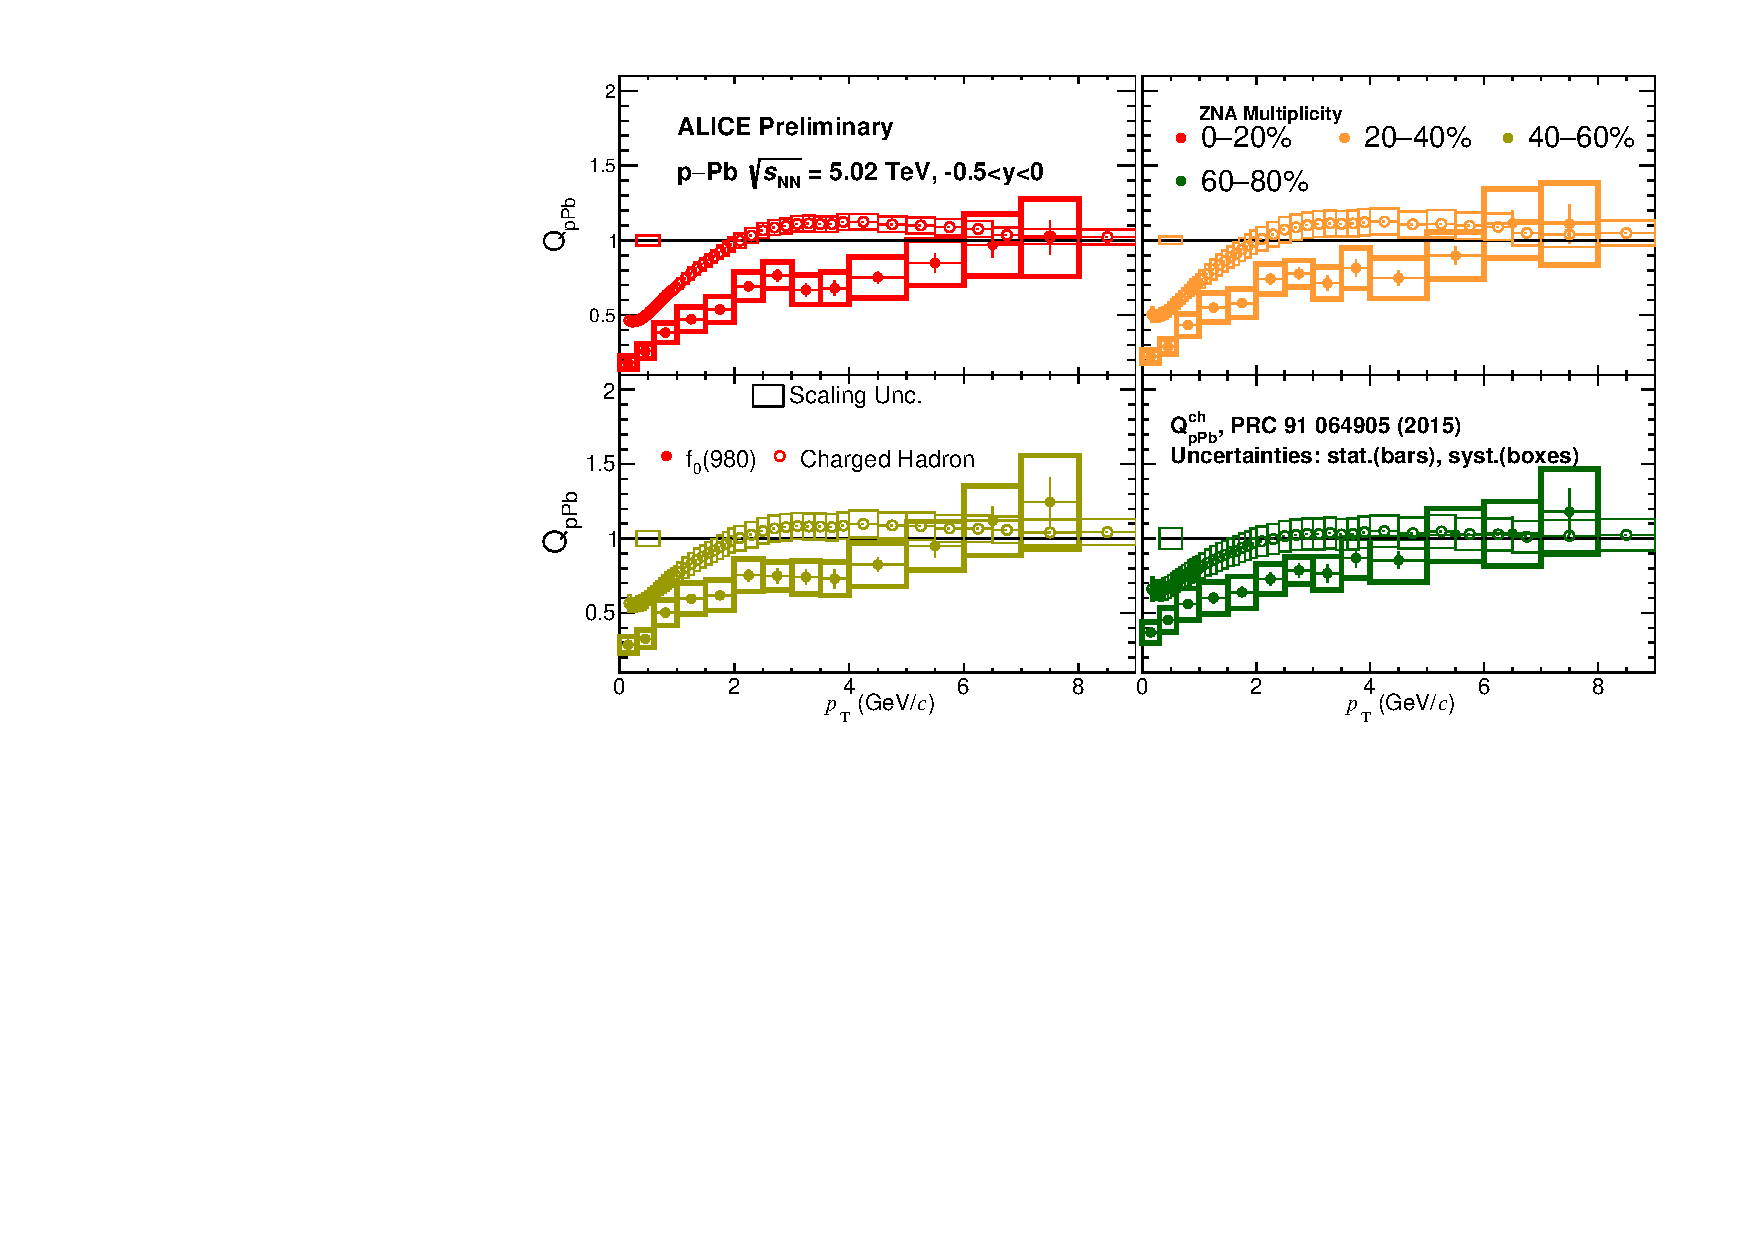
\includegraphics[width=0.8 \textwidth]{figures/Fig7_QpPb.pdf} }
	\caption{ Nuclear modification factor ($Q_{\rm{pPb}}$) of \fzero~as a function of $p_{\rm{T}}$ in p--Pb collisions at \snn~=~5.02~TeV for different multiplicity classes. Statistical and systematic uncertainties are shown as error bars and boxes, respectively. Open boxes around $p_{\rm{T}}$~=~0.5~GeV/$c$ represent the binary collision scaling uncertainties. The $Q_{\rm{pPb}}$ of \fzero~is compared with $Q_{\rm{pPb}}$~of charged hadrons. }
	\label{fig:QpPb}
\end{figure}

The $p_{\rm{T}}$-differential invariant yield of \fzero in p--Pb collisions can be compared to the one in pp collisions at the same center-of-mass energy by computing the nuclear modification factor $Q_{\mbox{pPb}}$, defined as 
\begin{eqnarray}
Q_{\mbox{pPb}} = \dfrac{\mathrm{d}^{2} N_{\mathrm{f}_{0}(980)}^{\mathrm{pPb}} / \mathrm{d} p_{\mathrm{T}} \mathrm{dy} }{ \left\langle T_{\mathrm{pPb}} \right\rangle \mathrm{d}^{2} \sigma_{\mathrm{f}_{0}(980)}^{\mathrm{pp}}/ \mathrm{d} p_{\mathrm{T}} \mathrm{dy} },
\end{eqnarray}
where $\left\langle T_{\mathrm{pPb}} \right\rangle$ and $\sigma_{\mathrm{f}_{0}(980)}^{\mathrm{pp}}$ are the average nuclear overlap from the Glauber model~\cite{Miller:2007ri} and the cross section for the production of \fzero~in pp collisions~\cite{ALICE:2022qnb}, respectively. Note that the B.R. is cancelled out in the measurement of the $Q_{\mbox{pPb}}$ as the same value is used in pp and p--Pb collisions.

Figure~\ref{fig:QpPb} shows the $Q_{\mbox{pPb}}$ of \fzero~in p--Pb collisions at \snn~=~5.02~TeV in different multiplicity classes. The Pb-remnant side ZN is used to select centrality intervals to calculate the $Q_{\mathrm{pPb}}$, which is described in Sec.~\ref{sec:setup}. The systematic uncertainties are calculated with the assumption that there is no correlated uncertainty between the yield in pp and p--Pb collisions. The \fzero~is more suppressed than charged hadrons in all measured centrality intervals for $p_{\mathrm{T}}<$~4~GeV/$c$. As $p_{\mathrm{T}}$ increases, $Q_{\rm{pPb}}$ becomes compatible and reaches unity for both cases. This result is consistent with the suppression shown in Fig.~\ref{fig:f0piPt}, indicating the strong suppression at low $p_{\mathrm{T}}$ and no suppression observed at high $p_{\mathrm{T}}$. In addition, the $Q_{\rm{pPb}}$ does not exhibit Cronin peak~\cite{Cronin:1974zm} at the intermediate $p_{\mathrm{T}}$ in HM events. This is consistent trend of conventional mesons. No Cronin peak for \fzero~might suggests that the number of constituent quarks of \fzero~is smaller than three.